\subsection{Apparatus}
\label{apparatus}

{\bf [add something on the variability of frequency range across subjects \cite{I don't remember}]}

{\bf [entropy covers the full range of power spectrum]}

{\bf [take passive watching as the default mode (not resting state which is not a natural state, during the day and when being in interaction with the outside world)]}

{\bf [comfort zone for RSVP reading is around 5-12 words per second and allows to easily follow the story \cite{kujala2007phase}]}


{\bf [blink artifacts $\rightarrow$ Szibbo, D., Luo, A. \& Sullivan, T. J. Removal of blink artifacts in single channel EEG. Conf. Proc. IEEE Eng Med. Biol. Soc. 2012, 3511�3514 (2012).]}

We shall now design a system that takes cognitive activity, recorded by  EEG and represented by entropy, as an input to control the speed, and the evolution of speed (resp. the first and second derivatives of instant display time) at which words are displayed on the screen through RSVP.

We define $X = X(t)$ the presentation duration for each word. At each iteration, X is updated according to,
% $\dot{x} = dx/dt$, the instant change of presentation duration, and $\ddot{x} = d\dot{x}/dt = d^{2}x/dt$, the instant change of  $\dot{x}$.  $\dot{x}$ and $\ddot{x}$ shall be seen as the speed and the acceleration of the presentation duration over time. These metrics are the control parameters of the brain speed reader, and shall help validate the hypotheses formulated above.

\begin{equation}
X(t+\Delta t) = X(t) \left[1 + \alpha \cdot S_{norm}(t)\right].
\label{eq:RateChange}
\end{equation}

with $S_{norm}$, the normalized entropy, continually updated according to (\ref{eq:Snormalized}), which is a well-centered, Gaussian-like, distribution with average $0$, by definition. $\alpha$ is a fixed parameter which determines the negative (resp. positive) incremental influence of $S_{norm}$ on $X(t)$. If $\alpha < 0$ and $S_{norm} > 0$ (reflecting higher cognitive activity), the pace of word display decreases. Conversely, if $\alpha > 0$ and $S_{norm} > 0$, then the pace of word display increases for higher cognitive activity computed from the power spectrum density, and measured every quarter second from the EEG.

Figure \ref{fig:apparatus} exhibits the apparatus and its step-by-step functioning: (i) the EEG signal is recorded, (ii)  processed online every quarter second  to obtain a power spectrum density, which is in turn (iii) represented by the normalized entropy  $S_{norm}$; (iv) depending on the values of parameter $\alpha$ and the random variable $S_{norm}$, the {\it brain speed reader} will change the pace of word rapid serial visual presentation.

The power spectrum varies as a function of the mental tasks occurring, but also as a result of potential external perturbations, such as eye-movement and blinking as well as muscle movements. During the brain speed reader experiment and preliminary tasks, subjects sit quietly in front of a screen. Nevertheless, to account for large perturbations arising from movements, we have implemented a simple quality check. If the median value of the EEG signal is superior to $150\mu s$, the measure of entropy $S$ is dropped, and the rate $X(t)$ is not updated. Separating sentences and paragraphs with small pauses is crucial to let subjects gain better understanding of the whole text \cite{}. After each sentence (resp. paragraph), we added the equivalent time of two (resp. four) words. For example, if the current rate is 150ms/word, then a pause of 300ms is used as a break between two sentences.

The parameter $\alpha$ is directly associated with the working hypotheses formulated above, which relate cognitive activity, neural synchronization and the most comfortable pace for an efficient RSVP. The sign of $\alpha$ helps test {\bf Hypothesis 1a}: words influence cognitive activity ($\alpha > 0$), and {\bf Hypothesis  1b}: cognitive activity constrains the ability to integrate and conceptualize knowledge ($\alpha  > 0$). The absolute value of $\alpha$ is a good test for {\bf Hypotheses 2}: the further $|\alpha|�\gg 0$, the more adaptive the process given by (\ref{eq:RateChange}).

\begin{figure}[!t]
\centering
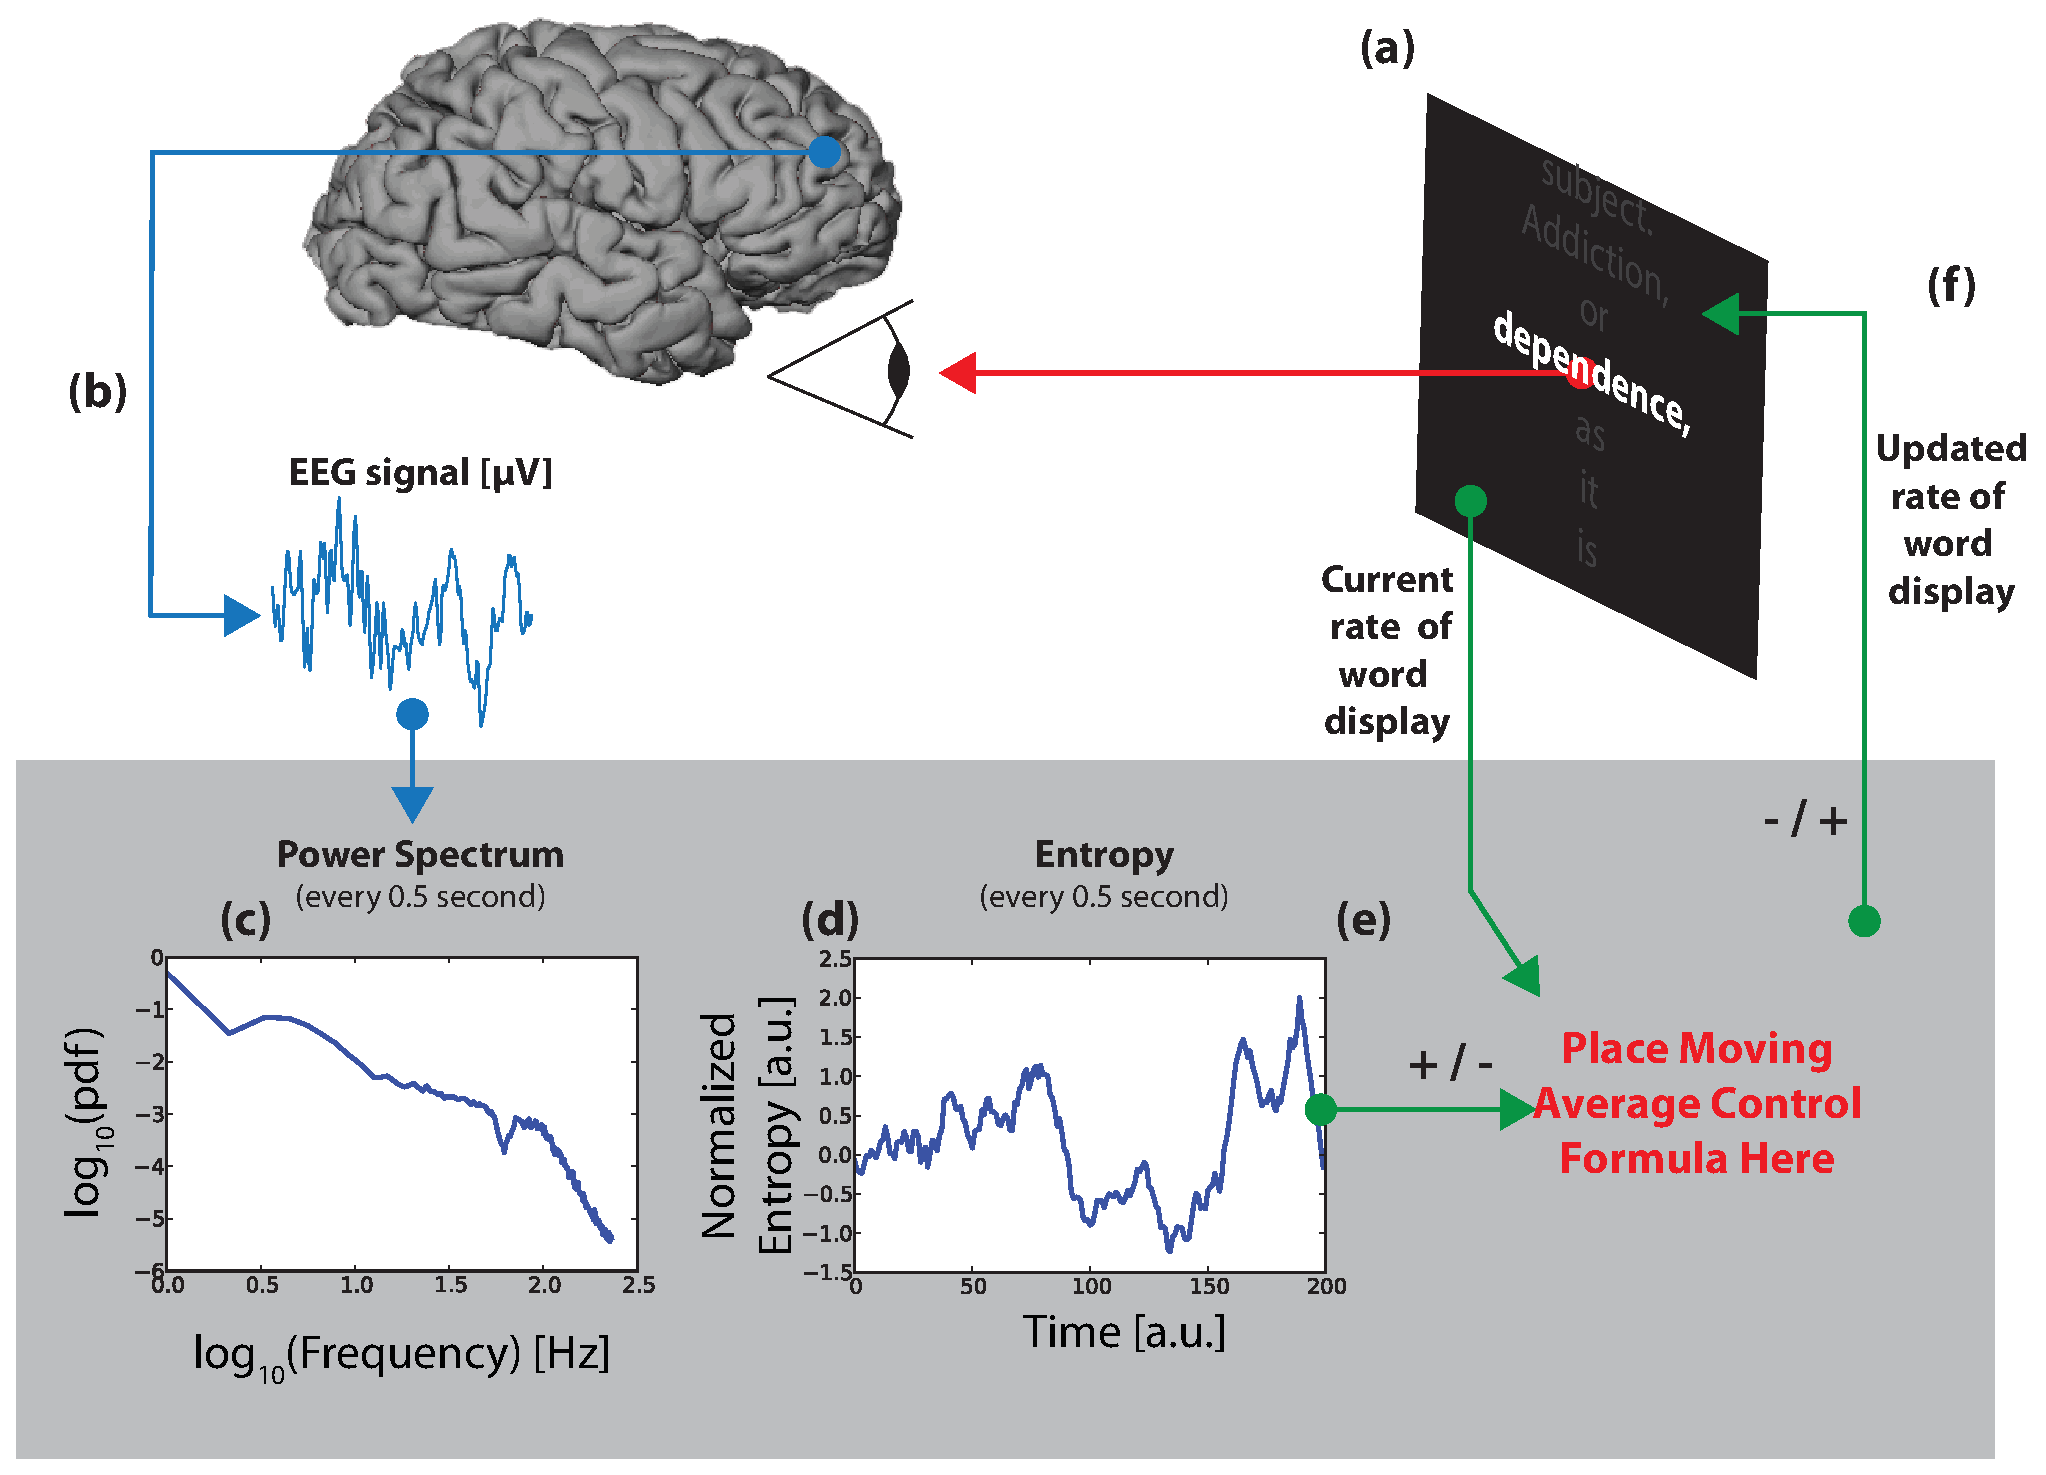
\includegraphics[width=0.9\columnwidth]{../figures/apparatus.eps}
\caption{Brain speed-reader apparatus: {\bf (a)} Words are displayed and read one after the other at a given rate. {\bf (b)} the EEG signal is recorded through a consumer grade device (here the {\it Neurosky Mindwave}). {\bf (c)} The EEG signal is turned every 0.5 seconds into a power spectrum through a Fourier transform, {\bf (d)} the characteristics of the power spectrum are compressed into a single value characteristic entropy $s$ value. {\bf (e)} A new rate of word display is updated by taking into its current value and $s$. {\bf (f)} The rate of word display is updated accordingly.}
\label{fig:apparatus}
\end{figure}
